\documentclass[12pt]{article}
\usepackage{hyperref}
\usepackage[pdftex]{graphicx}
\usepackage{multirow}
\usepackage{setspace}
\usepackage{color}
\usepackage{multicol}

\usepackage{listings}

\usepackage{textcomp}

\usepackage[T1]{fontenc} 


\hypersetup{
    bookmarks=true,         % show bookmarks bar?
    unicode=false,          % non-Latin characters in Acrobat’s bookmarks
    pdftoolbar=true,        % show Acrobat’s toolbar?
    pdfmenubar=true,        % show Acrobat’s menu?
    pdffitwindow=false,     % window fit to page when opened
    pdfstartview={FitH},    % fits the width of the page to the window
    pdftitle={My title},    % title
    pdfauthor={Author},     % author
    pdfsubject={Subject},   % subject of the document
    pdfcreator={Creator},   % creator of the document
    pdfproducer={Producer}, % producer of the document
    pdfkeywords={keyword1, key2, key3}, % list of keywords
    pdfnewwindow=true,      % links in new PDF window
    colorlinks=true,       % false: boxed links; true: colored links
    linkcolor=red,          % color of internal links (change box color with linkbordercolor)
    citecolor=green,        % color of links to bibliography
    filecolor=magenta,      % color of file links
    urlcolor=blue           % color of external links
}

% ME4140 - Fall 2016 - Fall2017

\textwidth=6.5in
\topmargin=-0.5in
\textheight=9.25in
\hoffset=-0.5in
\footskip=0.2in

\pagestyle{myheadings}
\markright{{\large ME 4140 Fall 2019---The Robotic Operating System}}

\definecolor{dkgreen}{rgb}{0,0.6,0}
\definecolor{gray}{rgb}{0.5,0.5,0.5}
\definecolor{mauve}{rgb}{0.58,0,0.82}

\definecolor{mygray}{rgb}{.6, .6, .6}
\definecolor{mypurple}{rgb}{0.6,0.1961,0.8}
\definecolor{mybrown}{rgb}{0.5451,0.2706,0.0745}
\definecolor{mygreen}{rgb}{0, .39, 0}

\newcommand{\R}{\color{red}}
\newcommand{\B}{\color{blue}}
\newcommand{\BR}{\color{mybrown}}
\newcommand{\K}{\color{black}}
\newcommand{\G}{\color{mygreen}}
\newcommand{\PR}{\color{mypurple}}

\newcommand{\pkgname}{\G<package\_name>\K}
\newcommand{\wspname}{\R<workspace\_name>\K}
\newcommand{\nodname}{\PR<node\_name>\K}
\newcommand{\tpcname}{/topic\_name}
\newcommand{\home}{\textasciitilde/}

\newcommand{\rosdistro}{kinetic}

\begin{document}

\thispagestyle{plain}

\begin{center}
   {\bf \Large ROS - Basics of Nodes and Topics}\vspace{2mm} \\
   {\bf \large ME 4140 - Introduction to Robotics - Fall 2019} \vspace{5mm}\\
\end{center}


\begin{description}

    \item [I. Components] The major building blocks of a ROS system

        \begin{enumerate}
                
            \item \href{http://wiki.ros.org/Master}{Master Node}
                \begin{itemize}
                    \item {\it The ROS Master provides naming and registration services to the rest of the nodes in the ROS system.}** 
                    \item master node runs first  {\fontfamily{qcr}\selectfont  \hspace{5mm} \$ roscore } \\
                    \item core of the system or robot {\fontfamily{qcr}\selectfont  \hspace{5mm} \$ ROS\_MASTER\_URI=http://12345 } \\
                    

                \end{itemize}
            
            \item \href{http://wiki.ros.org/Nodes}{Nodes}             
                \begin{itemize}
                    \item {\it A node is a process that performs computation.}** 
                    \item each 'program' or 'element' of the robot is a node\\examples:
                        \begin{itemize} 
                        \begin{multicols}{2}    
                        
                            \item sensor
                            \item hardware driver    
                            \item navigation 
                            \item keyboard or joystick        
                            
                        \end{multicols}
                        \end{itemize}
                    \item start or run node individually after master\vspace{5mm}\\
                    {\fontfamily{qcr}\selectfont  \hspace{5mm} \$ rosrun <packagename> <nodename> <options> } \vspace{1mm}\\
                  
                    \item all nodes are registered to the master and communicate in different ways
                        \begin{itemize}
                            \item  \href{http://wiki.ros.org/Topics}{topics} - publishing and subscribing
                            \item \href{http://wiki.ros.org/Parameter%20Serverparameters}{parameter server} - static data
                            \item \href{http://wiki.ros.org/Services}{services} - subroutine call
                        \end{itemize}    
                                      
                \end{itemize}
                
            \item \href{http://wiki.ros.org/Packages}{Packages} 

                \begin{itemize}
                    \item {\it Software in ROS is organized in packages. A package might contain ROS nodes, a ROS-independent library, a dataset, configuration files, a third-party piece of software, or anything else that logically constitutes a useful module.}** 
                    \item a collection of related nodes, each node belongs to a package
                                     
                    \item pre-built packages available with ros installation {\fontfamily{qcr}\selectfont  \hspace{5mm} -desktop-full}
                    \item pre-built packages available for installation \\
                    \begin{description}
                        \item[apt-get] {\fontfamily{qcr}\selectfont  \hspace{1mm} \$ sudo apt-get install ros-<distribution>-<packagename> } 
                        \item[rosdep]{\fontfamily{qcr}\selectfont  \hspace{1mm} \$ rosdep install <packagename> } \\
                    \end{description}
                    \item update ubuntu before installing anything \\
                    {\fontfamily{qcr}\selectfont  \hspace{2mm} \$ sudo apt-get update } \\
                    {\fontfamily{qcr}\selectfont  \hspace{2mm} \$ sudo apt-get check }                
                \end{itemize}            

                
                
    \end{enumerate}
    ** from (ros.org)
    \newpage
    
    \item [II. The Graph of the System] ROS works on a system of interconnected nodes. It is very useful to visualize this in a graph.\\
        \begin{enumerate}   
            
            \item \href{http://wiki.ros.org/rqt_graph}{RQT Graph} A very useful tool. A node {\it rqt\_graph} in a package {\it rqt\_graph}. \\\\
                    {\fontfamily{qcr}\selectfont  \hspace{5mm} \$ rosrun rqt\_graph rqt\_graph}\\
            
            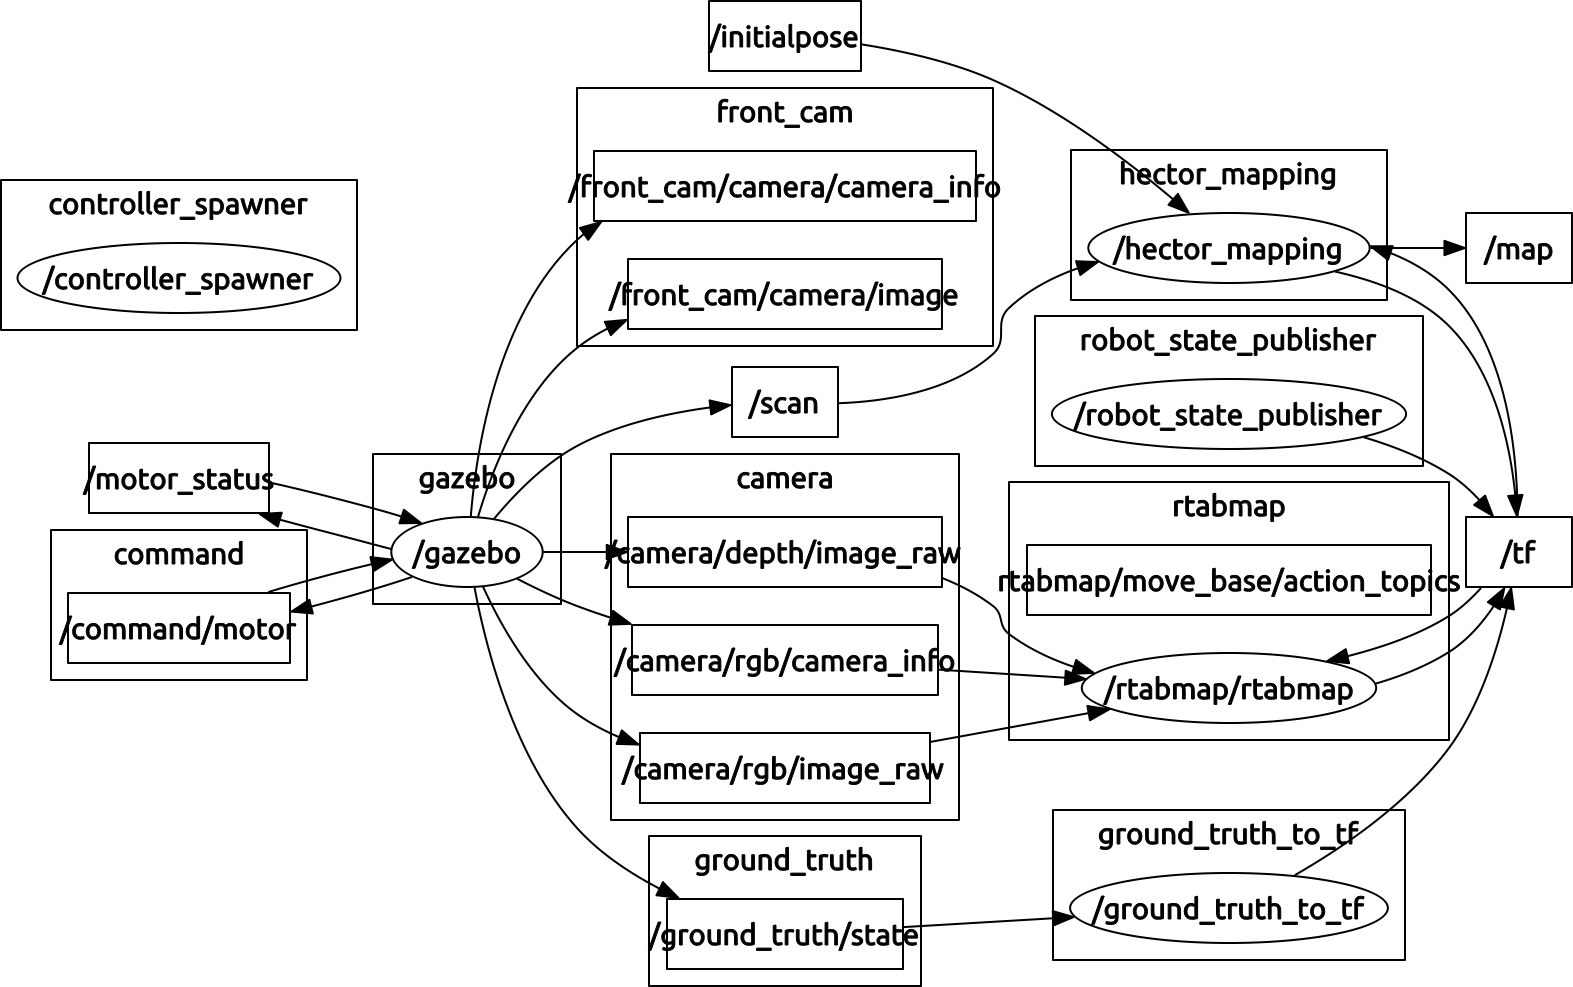
\includegraphics[scale=.4]{ros_basics_fig1.png} \\
            
            \item \href{http://wiki.ros.org/rqt_plot}{RQT Plot} A very useful tool. A node {\it rqt\_plot} in a package {\it rqt\_plot}. \\
                {\fontfamily{qcr}\selectfont  \hspace{5mm} \$ rosrun rqt\_plot rqt\_plot}\\
            
            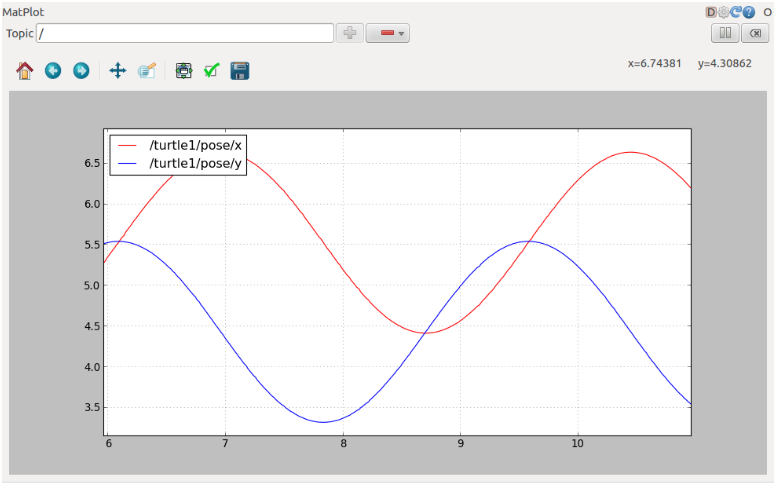
\includegraphics[scale=.5]{ros_basics_fig2.png} \\    
          \end{enumerate}       


\newpage
    
    \item [III. Topics, Publishers, and Subscribers] The nodes in a ROS system communicate.  
        \begin{enumerate}   
           \item \href{http://wiki.ros.org/Topics}{Topics} 
                    \begin{itemize}
                        \item data available to nodes in the system
                        \item each topic has a name    
                        \item data is stored and transferred in standard ros data types
                        \item generally data is streaming, but does not have to be
                    \end{itemize}    
           \item \href{http://wiki.ros.org/ROS/Tutorials/WritingPublisherSubscriber(c++)}{Publishers}
                    \begin{itemize}
      
                        \item data produced by a node can be shared with the system by publishing a topic
                        \item a node which outputs topic data is a publisher
                        \item a node may publish multiple topics 
                        
                        \end{itemize}  
            \item \href{http://wiki.ros.org/ROS/Tutorials/WritingPublisherSubscriber(c++)}{Subscribers}
                \begin{itemize}
      
                        \item a registered node can access the data in a topic by subscribing to a topic
                        \item a node which gets topic data as input is a subscriber
                        \item a node may subscribe to multiple topics 
                    \end{itemize}  
                    
            \item \href{http://wiki.ros.org/rostopic}{rostopic}                    
                \begin{itemize}   
                    \item a very useful tool, a built in package 
                    \item used differently than other packages, does not require rosrun
                    \item a set of different tools
                    \begin{description}   
                        \item [list] {\fontfamily{qcr}\selectfont  \hspace{5mm} \$ rostopic list}\\
                        \item [echo] {\fontfamily{qcr}\selectfont  \hspace{5mm} \$ rostopic echo /topicname}\\
                        \item [type] {\fontfamily{qcr}\selectfont  \hspace{5mm} \$ rostopic pub /topicname}\\
                    \end{description}  
                \end{itemize}    
                    \item  \href{http://wiki.ros.org/msg}{data types} - topics are published in standard types called messages
                    \begin{itemize}
                        \item {\fontfamily{qcr}\selectfont  \hspace{5mm} std\textunderscore msgs/int32 }
                        \item {\fontfamily{qcr}\selectfont  \hspace{5mm} std\textunderscore msgs/float32 }\\
                        
                        \item {\fontfamily{qcr}\selectfont  \hspace{5mm} geometry\textunderscore msgs/Point }
                        \item {\fontfamily{qcr}\selectfont  \hspace{5mm} geometry\textunderscore msgs/Pose }\\
                        
                        \item {\fontfamily{qcr}\selectfont  \hspace{5mm} nav\textunderscore msgs/Odometry }
                        \item {\fontfamily{qcr}\selectfont  \hspace{5mm} nav\textunderscore msgs/Path }\\
                    \end{itemize}
                    
                    \item let show an example now!
                                      
        \end{enumerate}     
\newpage
    
%    \item [IV. Services] The nodes in a ROS system can also communicate through services. Thsi is for reply/request type operations.  
%  \begin{enumerate} 
%\item \href{http://wiki.ros.org/Services}{Services}
%\end{enumerate}    
%\newpage
    
    \item [IV. A Simple Robot Simulator] : \\
        \begin{enumerate}    
            \item Update and Install  \href{http://wiki.ros.org/turtlesim}{turtlesim}.  \\
			
			{\bf \texttt{\$ sudo apt-get update }} \\\\
			
			{\bf \texttt{\$ sudo apt-get install ros-melodic-turtlesim } }\\\\
	\item Start the core. \\\\	 

			{\bf \texttt{\$ roscore} }\\\\
			
			\item Open a new terminal window.\\\\
			
			{\bf \texttt{\$ rosrun turtlesim turtlesim\_node} }\\\\
			
			{\bf \texttt{\$ rostopic list} }\\ \\
			
			\item Now lets add a controller node.\\\\
			
			
			{\bf \texttt{\$ sudo apt-get install ros-kinetic-teleop-twist-keyboard}}\\\\
			
			{\bf \texttt{\$ rosrun teleop\_twist\_keyboard teleop\_twist\_keyboard.py }}\\\\
			
			\item There is a problem, we need to make sure the nodes are talking. Add the following {\it options} to the end of the previous command and rerun the node. \\\\
			
			{\bf \texttt{/cmd\_vel:=/turtle1/cmd\_vel }}\\\\
			
        \end{enumerate}  
\end{description}
\end{document}

